\documentclass[]{beamer}
%Information to be included in the title page:
% -*-coding: utf-8 -*-
%%***********************************************
%% Plantilla para TFG.
%% Escuela Técnica Superior de Ingenieros Informáticos. UPM.
%%***********************************************
%% Preámbulo del documento.
%%***********************************************
\usepackage[utf8]{inputenc}
\usepackage[T1]{fontenc}
\usepackage[english,spanish,es-lcroman]{babel}
\usepackage{bookman}
\decimalpoint
\usepackage{graphicx}
\usepackage{bookmark}
\usepackage{amsfonts,amsgen,amsmath,amssymb}
\usepackage[top=3cm, bottom=3cm, right=2.54cm, left=2.54cm]{geometry}
\usepackage{afterpage}
\usepackage{colortbl,longtable}
\usepackage{hyperref} 
\usepackage{pdfpages}
\usepackage{url}
\usepackage{multicol}
\usepackage[stable]{footmisc}
\usepackage{parskip} % para separar párrafos con espacio.
%%-----------------------------------------------
\usepackage{fancyhdr}
\pagestyle{fancy}
\fancyhf{}
\fancyhead[LO]{\leftmark}
\fancyhead[RE]{\rightmark}
\setlength{\headheight}{1.5\headheight}
\cfoot{\thepage}

\addto\captionsspanish{ \renewcommand{\contentsname}
  {Tabla de contenidos} }
\setcounter{tocdepth}{4}
\setcounter{secnumdepth}{4}

\renewcommand{\chaptermark}[1]{\markboth{\textbf{#1}}{}}
\renewcommand{\sectionmark}[1]{\markright{\textbf{\thesection. #1}}}
\newcommand{\HRule}{\rule{\linewidth}{0.5mm}}
\newcommand{\bigrule}{\titlerule[0.5mm]}

\usepackage{appendix}
\renewcommand{\appendixname}{Anexos}
\renewcommand{\appendixtocname}{Anexos}
%\renewcommand{\appendixpagename}{Anexos}
%%-----------------------------------------------
%% Páginas en blanco sin cabecera:
%%-----------------------------------------------
\usepackage{dcolumn}
\newcolumntype{.}{D{.}{\esperiod}{-1}}
\makeatletter
\addto\shorthandsspanish{\let\esperiod\es@period@code}

\def\clearpage{
  \ifvmode
    \ifnum \@dbltopnum =\m@ne
      \ifdim \pagetotal <\topskip
        \hbox{}
      \fi
    \fi
  \fi
  \newpage
  \thispagestyle{empty}
  \write\m@ne{}
  \vbox{}
  \penalty -\@Mi
}
\makeatother
%%-----------------------------------------------
%% Estilos código de lenguajes: Consola, C, C++ y Python
%%-----------------------------------------------
\usepackage{xcolor}

\definecolor{gray97}{gray}{.97}
\definecolor{gray75}{gray}{.75}
\definecolor{gray45}{gray}{.45}

\usepackage{listings}
\lstset{ frame=Ltb,
     framerule=0pt,
     aboveskip=0.5cm,
     framextopmargin=3pt,
     framexbottommargin=3pt,
     framexleftmargin=0.4cm,
     framesep=0pt,
     rulesep=.4pt,
     backgroundcolor=\color{gray97},
     rulesepcolor=\color{black},
     %
     stringstyle=\ttfamily,
     showstringspaces = false,
     basicstyle=\scriptsize\ttfamily,
     commentstyle=\color{gray45},
     keywordstyle=\bfseries,
     %
     numbers=left,
     numbersep=6pt,
     numberstyle=\tiny,
     numberfirstline = false,
     breaklines=true,
   }
\lstnewenvironment{listing}[1][]
   {\lstset{#1}\pagebreak[0]}{\pagebreak[0]}

\lstdefinestyle{consola}
   {basicstyle=\scriptsize\bf\ttfamily,
    backgroundcolor=\color{gray75},    
    }

\lstdefinestyle{CodigoC}
   {basicstyle=\scriptsize,
	frame=single,
	language=C,
	numbers=left
   }
   
\lstdefinestyle{CodigoC++}
   {basicstyle=\small,
	frame=single,
	backgroundcolor=\color{gray75},
	language=C++,
	numbers=left
   }

\lstdefinestyle{Python}
   {language=Python,    
   }

\lstdefinelanguage{yaml}
{
   keywords={true,false,null,y,n},
   keywordstyle=\bfseries,
   basicstyle=\bfseries,
   sensitive=false,
   captionpos=b,
   comment=[l]{\#},
   morecomment=[s]{/*}{*/},
   commentstyle=\ttfamily,
   stringstyle=\mdseries\ttfamily,
   moredelim=[l]{\&},
   moredelim=[l]{*},
   moredelim=**[il][\mdseries{:}\mdseries]{:},
   morestring=[b]',
   morestring=[b]",
   literate =  {---}{{\llap{\mdseries-{-}-}}}3    
               {|}{{\textbar}}1 
               {\ -\ }{{\mdseries\ -\ }}3,
}

\colorlet{punct}{red!60!black}
\definecolor{delim}{RGB}{20,105,176}
\colorlet{numb}{magenta!60!black}
\lstdefinelanguage{json}{
   basicstyle=\bfseries,
   captionpos=b,
   showstringspaces=false,
   breaklines=true,
   stringstyle=\mdseries\ttfamily,
   moredelim=[l]{\&},
   moredelim=[l]{*},
   moredelim=**[il][\mdseries{:}\mdseries]{:},
   morestring=[b]',
   morestring=[b]",
   frame=lines
}

\usepackage[textwidth=2.5cm, textsize=smaller]{todonotes}
\setlength{\marginparwidth}{2.5cm}

\usepackage{lipsum}

\usepackage{relsize}

%\includeonlyframes{intro,howto}
%\includeonlyframes{problemas,objetivos}
%\includeonlyframes{ansible,python,interfaz}
%\includeonlyframes{demo,trabajo_futuro,conclusiones}

\begin{document}

\frame{\titlepage}
\tableofcontents

\section{Introducción}
\subsection{¿Qué es Prometheus?}
\begin{frame}[label=intro]
    \frametitle{¿Qué es Prometheus?}
    \begin{columns}
        \begin{column}{0.6\textwidth}
            \begin{figure}[H]
                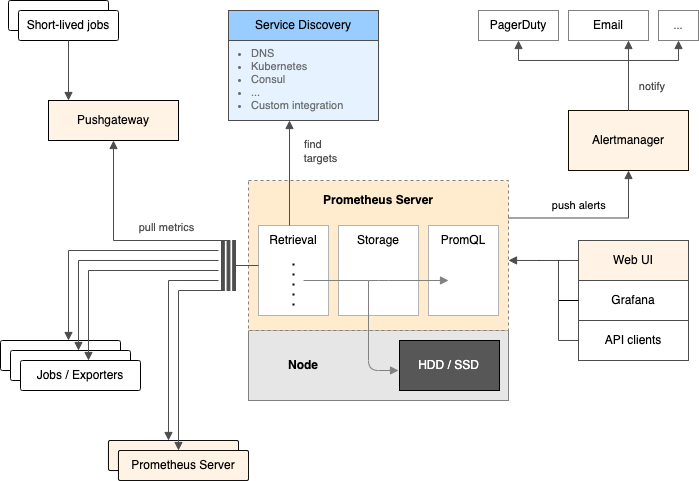
\includegraphics[width=\textwidth]{include/prometheus_arch.png}
                \caption{Arquitectura de funcionamiento de Prometheus}
            \end{figure}
        \end{column}
        \begin{column}{0.45\textwidth}
            \centering
            ¿Qué se necesita para monitorizar con Prometheus?
            \begin{itemize}
                \item Servidor de prometheus
                \item Targets con etiquetas,\\ agrupados por proyectos
                \item Reglas de alertado
            \end{itemize}
        \end{column}
    \end{columns}
    \input{secciones/notas/intro_prometheus_notes}
\end{frame}

\subsection{¿Cómo se monitoriza un nuevo target?}
\begin{frame}[label=howto,fragile]
    \frametitle{¿Cómo se monitoriza un nuevo target?}
    \begin{multicols}{2}
        Forma estática:
        \begin{verbbox}[\small\slshape]
- job: node exporter
  static_configs:
  - targets:
    - "localhost:9091"
      labels:
      jobname: node
      os: linux
        \end{verbbox}
        \noindent\hspace{1cm}\fbox{\theverbbox}
        \columnbreak
        
        Forma dinámica:
        \begin{verbbox}[\small\slshape]
- job: node exporter
  file_sd_configs:
  - files:
    - "targets/*.json"
    refresh_interval: 2m
        \end{verbbox}
        \noindent\hspace{1cm}\fbox{\theverbbox}
        \begin{verbbox}[\small\slshape]
{
  "targets": [
    "localhost:9091"
  ],
  "labels": {
    "jobname": "node",
    "os": "linux"
  }
}
        \end{verbbox}
        \noindent\hspace{1in}\fbox{\theverbbox}
    \end{multicols}
  \input{secciones/notas/howto_monitorizar_notes}
\end{frame}


\section{Motivaciones y Objetivos}
\subsection{Motivaciones: Problemas con la monitorización actual}
\begin{frame}[label=problemas]
    \frametitle{Motivaciones: Problemas con la monitorización actual}
    \begin{enumerate}
        \item Proceso lento y repetitivo
        \item Con etiquetas diferentes, hay que separar los targets
        \item No hay automatizaciones oficiales
        \item Alta probabilidad de introducir errores humanos
        \item Con ficheros grandes, los errores son difíciles de detectar
    \end{enumerate}

    \note{
    \begin{enumerate}
        \item Proceso lento y repetitivo
        \item Con etiquetas diferentes, hay que separar los targets
        \item No hay automatizaciones oficiales
        \item Alta probabilidad de introducir errores humanos
        \item Con ficheros grandes, los errores son difíciles de detectar
    \end{enumerate}
}
\end{frame}

\subsection{Objetivos: ¿Qué se pretende conseguir con la app?}
\begin{frame}[label=objetivos]
    \frametitle{Objetivos: ¿Qué se pretende conseguir con la app?}
    \begin{itemize}
        \item Automatizar el proceso de añadir targets
        \item Aumentar la rapidez y eficacia del proceso
        \item Disminuir el número de errores introducidos
    \end{itemize}
    \input{secciones/notas/objetivos_notes}
\end{frame}


\section{Proceso de desarrollo}
\subsection{Ansible}
Ansible\cite{ansible} es una herramienta de automatización, aprovisionamiento y configuración. Utiliza el protocolo SSH (aunque también puede utilizar otros como Kerberos o LDAP si fuera necesario) para realizar operaciones en las máquinas objetivo sin necesidad de tener un agente instalado en ellas.
\subsubsection{Inventario}
Ansible puede puede atacar a distintos nodos o \textit{hosts} al mismo tiempo. Para ello, lo más común es crear un listado de los mismos, agrupándolos según una serie de criterios, como por ejemplo:
\begin{itemize}
    \item Región
    \item Entorno (productivo, test, preproductivo, etc.)
    \item Funcionalidad (servidor web, base de datos, etc.)
\end{itemize}
De esta manera, un mismo \textit{host} puede estar incluido en varios grupos al mismo tiempo.

Además, también pueden especificarse distintas variables, que Ansible usará en la ejecución, tanto para cada \textit{host} como para cada grupo.

\subsubsection{Playbooks}
Los \textit{playbooks} son una forma de automatizar tareas repetitivas en las máquinas. En ellos se especifican una serie de tareas a realizar, y los \textit{hosts} en los que se ejecutará cada una. 

En este proyecto, se ha creado un playbook (ver \hyperref[lst:playbook]{Listing \ref{lst:playbook}}) que se encarga de instalar el agente \textit{node\_exporter} en las máquinas Linux que se especifiquen. Para ello, utiliza un rol de la comunidad de Ansible, que se encarga de realizar la instalación.



\subsection{API en Python}
\begin{frame}[label=python]
    \frametitle{API en Python}
    \begin{itemize}
        \item Establece el backend
        \item Genera endpoints para conectar con frontend
        \item Ejecuta ansible para instalar node exporter en los targets
        \item Ejecuta ansible para añadir target a Prometheus
        \item Crea el exporter de versiones en el target
        \item Añade un fichero de targets y de reglas de alertado\\ para cada proyecto
    \end{itemize}
    \input{secciones/notas/api_python_notes}
\end{frame}

\subsection{Interfaz}
\begin{frame}[label=interfaz]
    \frametitle{Interfaz}
    \begin{itemize}
        \item Hecha con ElectronJS
        \item Simple y práctica
        \item Permite:
        \begin{enumerate}
            \item Crear proyectos
            \item Añadir targets
            \item Buscar targets por projecto
        \end{enumerate} 
    \end{itemize}
    \input{secciones/notas/interfaz_notes}
\end{frame}


\section{Resultados y Conclusiones}
\subsection{Resultados: Funcionamiento de la aplicación}
\begin{frame}[plain,label=demo]
    \frametitle{Resultados: Funcionamiento de la aplicación}
    \begin{columns}
        \begin{column}{0.5\textwidth}
            \begin{figure}[H]
                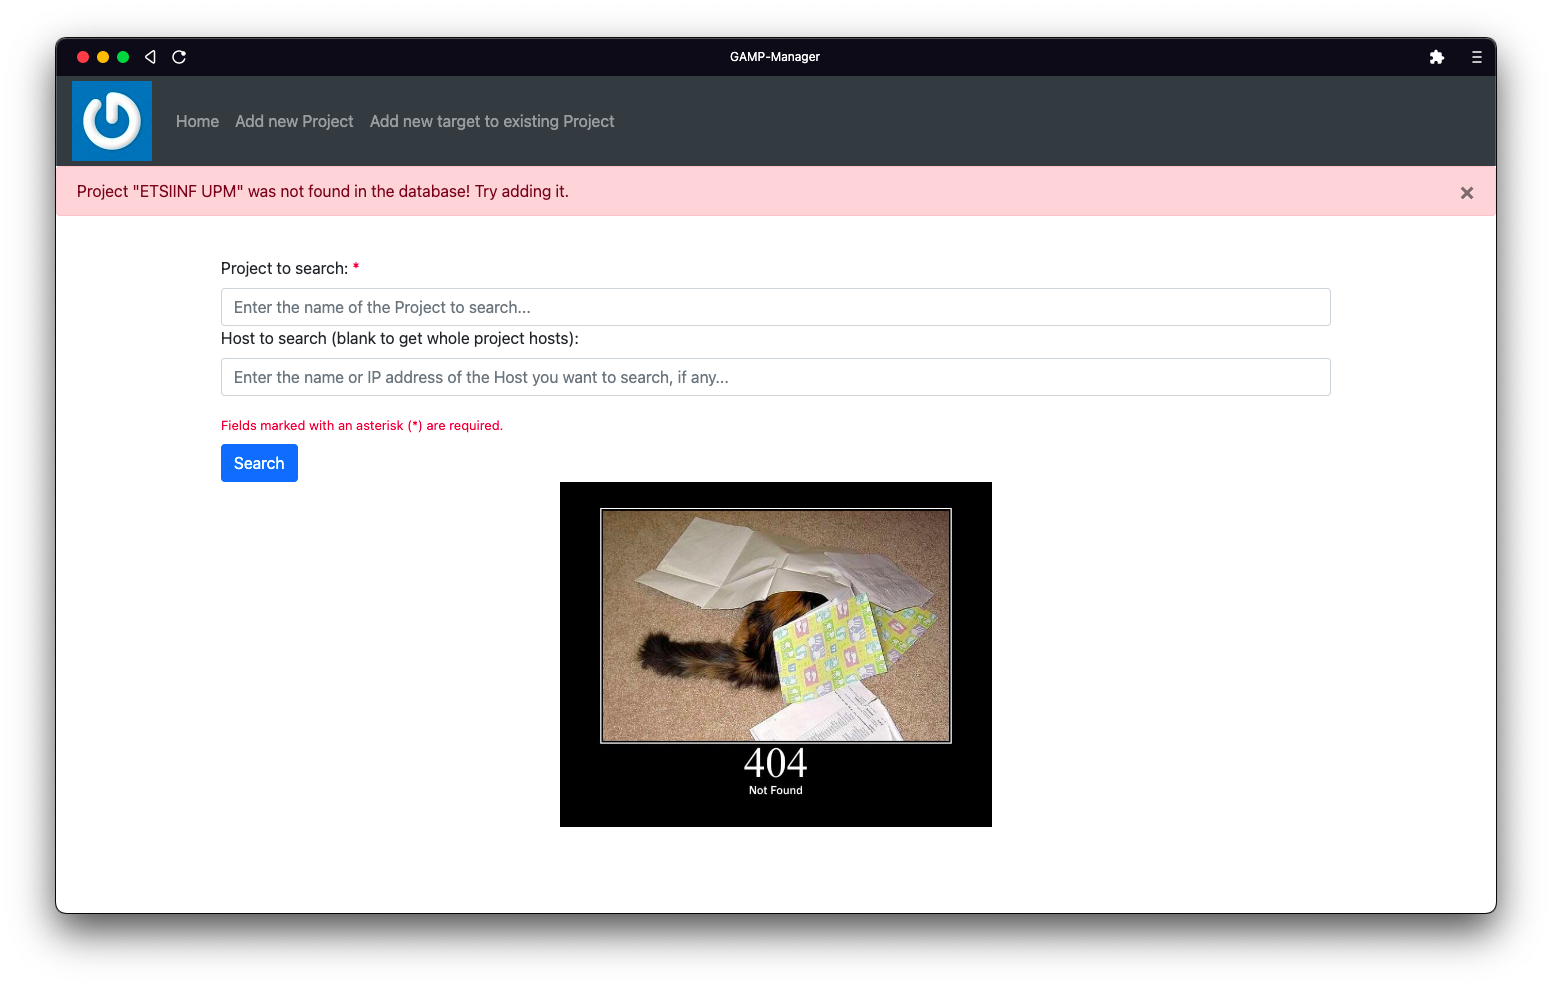
\includegraphics[width=\textwidth]{include/app_images/project_not_found.png}
            \end{figure}
        \end{column}
        \begin{column}{0.5\textwidth}
            \begin{figure}[H]
                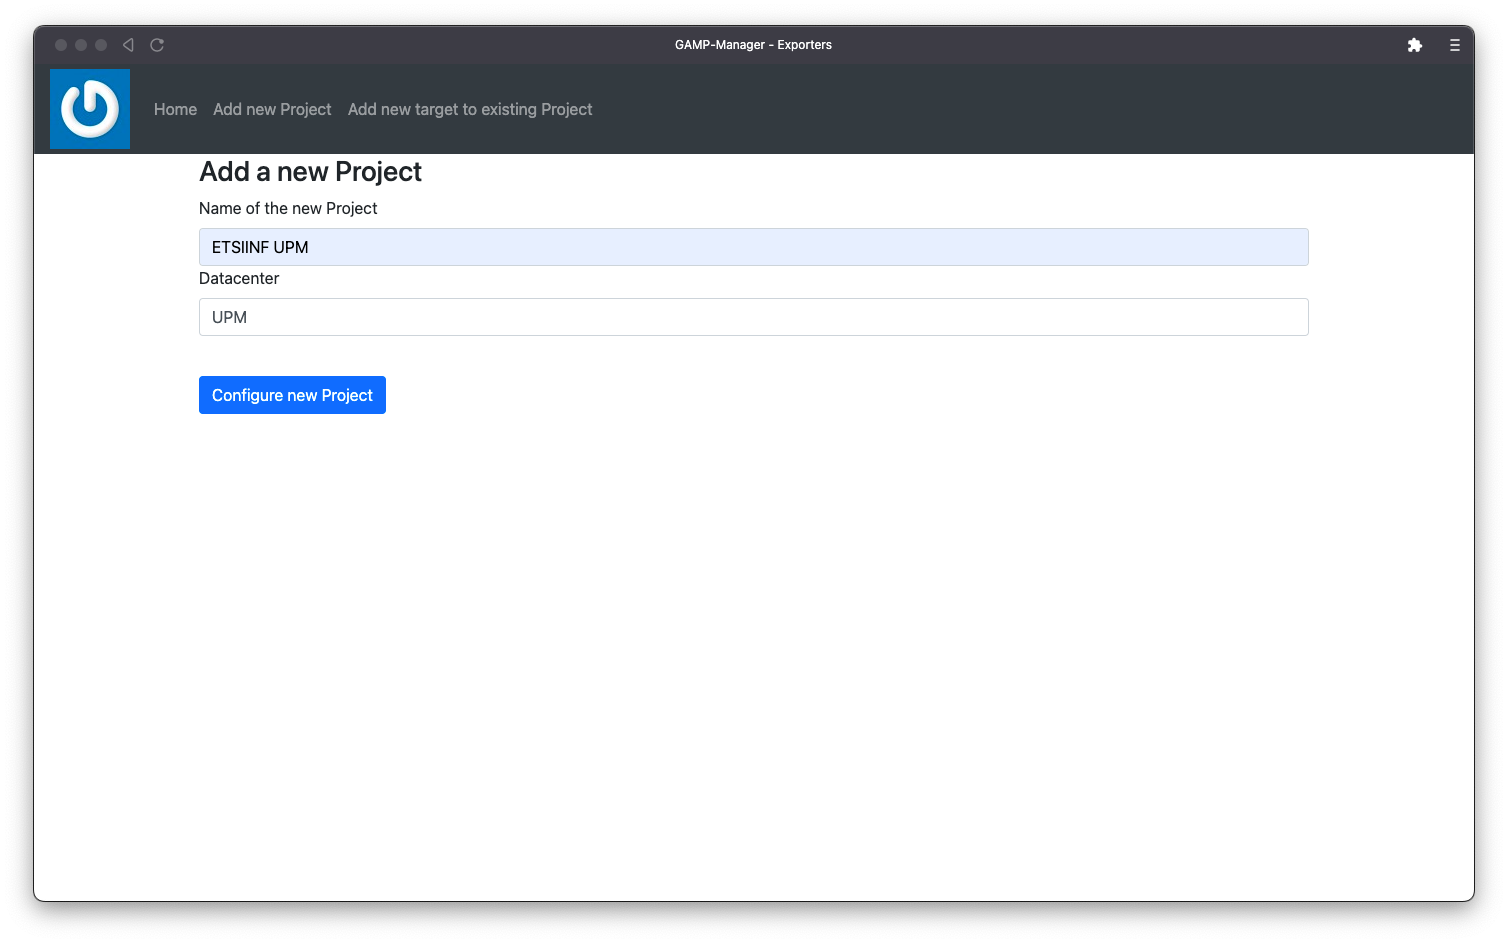
\includegraphics[width=\textwidth]{include/app_images/new_project.png}
            \end{figure}
        \end{column}
    \end{columns}
    \input{secciones/notas/demo_notes}
\end{frame}

\begin{frame}[plain,label=demo]
    \frametitle{Resultados: Funcionamiento de la aplicación}
    \begin{columns}
        \begin{column}{0.5\textwidth}
            \begin{figure}[H]
                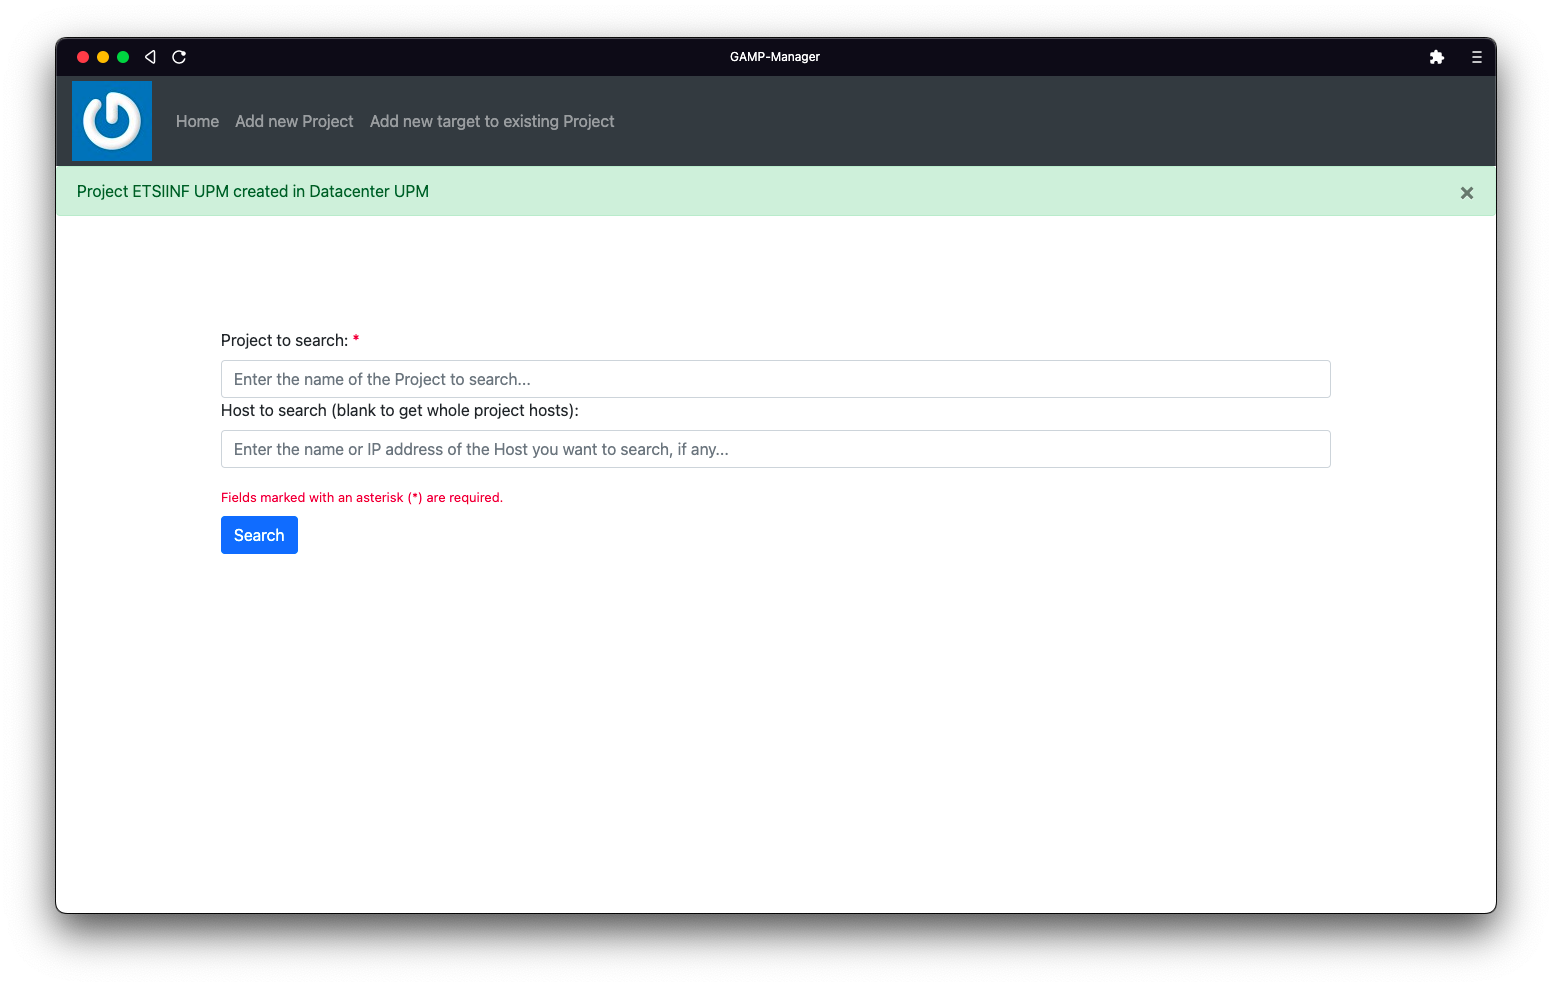
\includegraphics[width=\textwidth]{include/app_images/project_created.png}
            \end{figure}
        \end{column}
        \begin{column}{0.5\textwidth}
            \begin{figure}[H]
                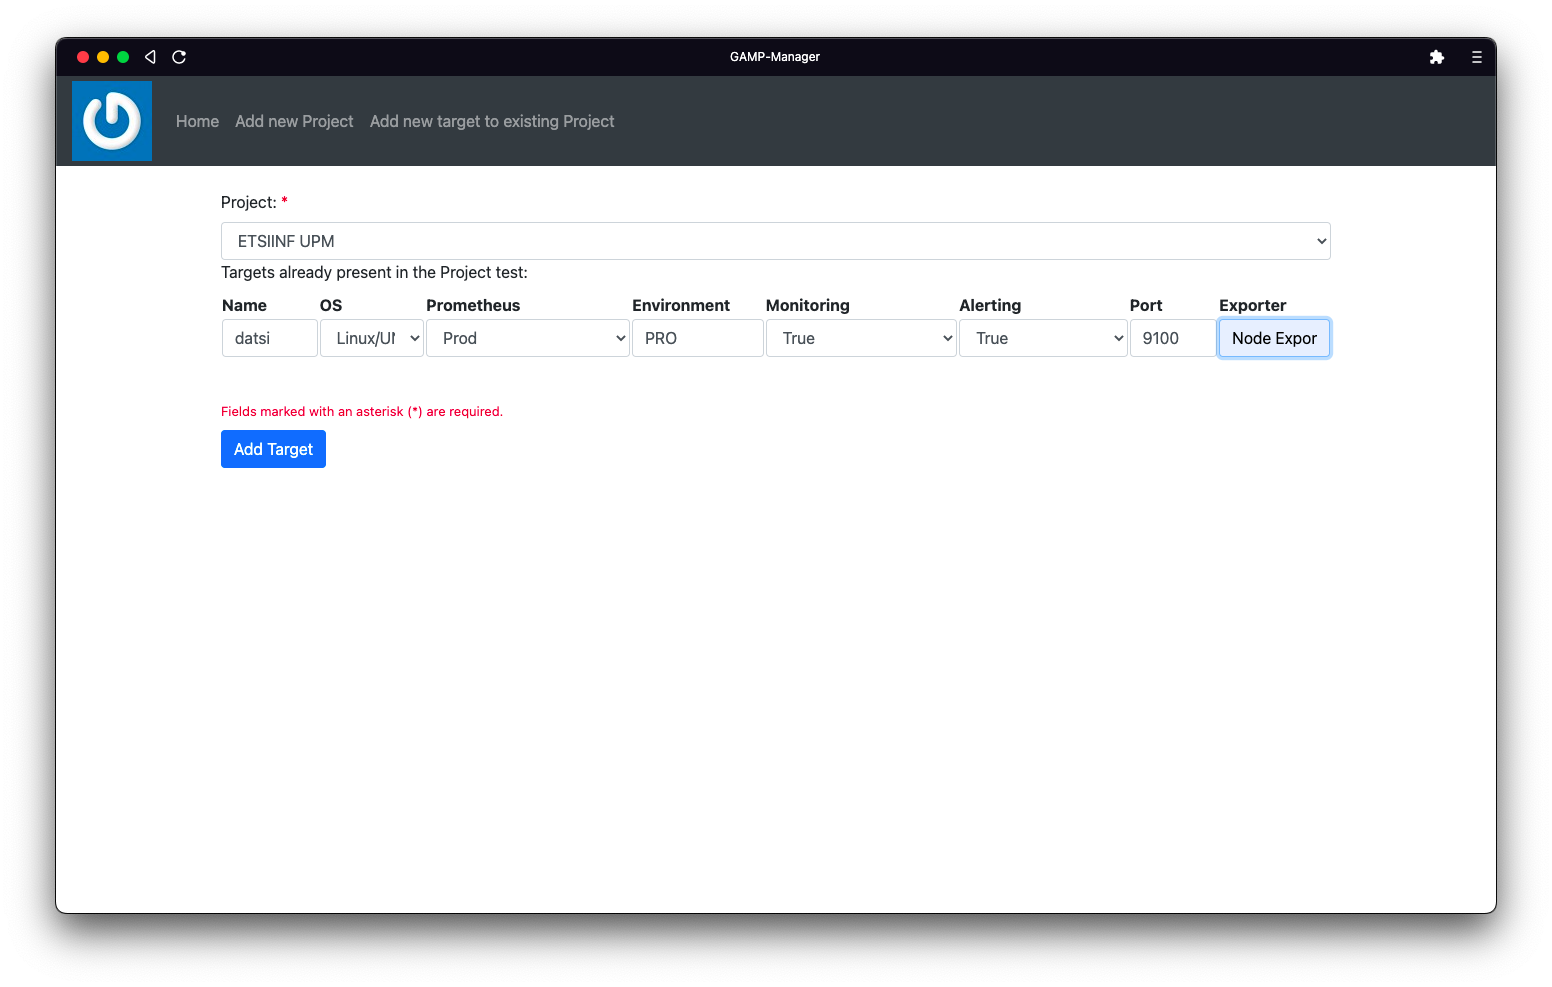
\includegraphics[width=\textwidth]{include/app_images/create_target.png}
            \end{figure}
        \end{column}
    \end{columns}
    \input{secciones/notas/demo_notes}
\end{frame}

\begin{frame}[plain,label=demo]
    \frametitle{Resultados: Funcionamiento de la aplicación}
    \begin{columns}
        \begin{column}{0.5\textwidth}
            \begin{figure}[H]
                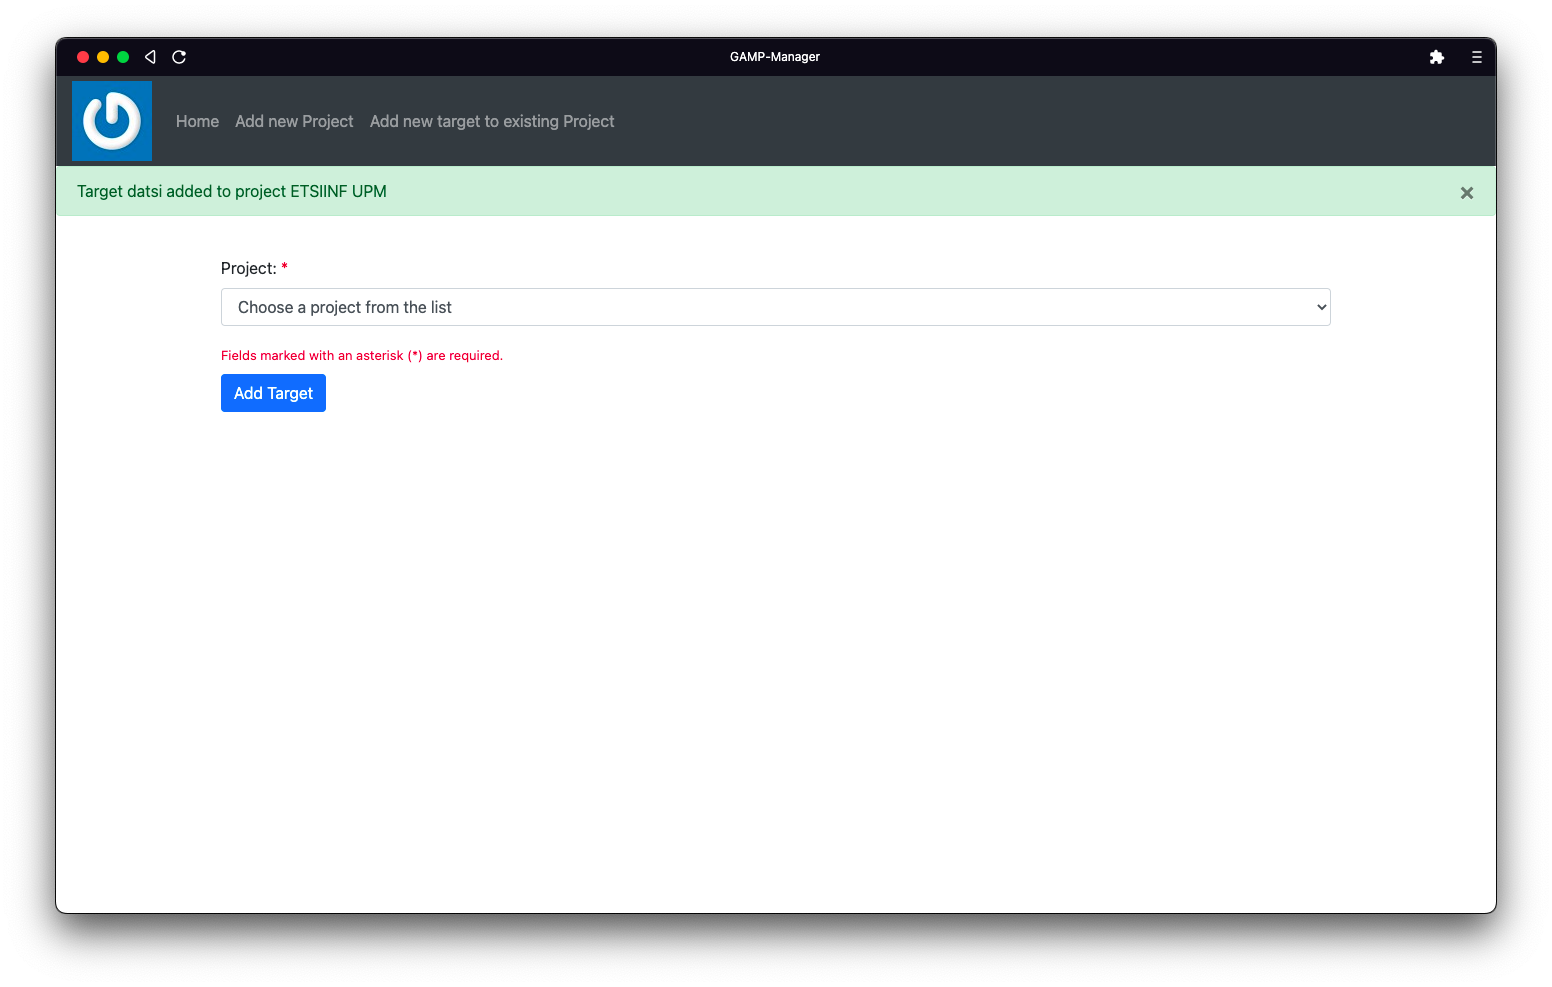
\includegraphics[width=\textwidth]{include/app_images/target_added.png}
            \end{figure}
        \end{column}
        \begin{column}{0.5\textwidth}
            \tiny
            \begin{verbatim}
$ tree .
.
|-- prometheus.yml
|-- rules
|   |-- cbgi_record_rules.yml
|   |-- standard.yml
|-- targets

2 directories, 3 files
\end{verbatim}
            
\begin{verbatim}
$ tree .
.
|-- prometheus.yml
|-- rules
|   |-- ETSIINF_UPM_alerts.yml
|   |-- cbgi_record_rules.yml
|   |-- standard.yml
|-- targets
    |-- ETSIINF_UPM.json

2 directories, 5 files
\end{verbatim}
        \end{column}
    \end{columns}
    \input{secciones/notas/demo_notes}
\end{frame}


\subsection{Trabajo futuro}
\begin{frame}[label=trabajo_futuro]
    \frametitle{Trabajo futuro}
    \begin{itemize}
        \item Trabajar con más exporters
        \item Añadir más servidores de Prometheus, Alertmanager y Grafana
        \item Monitorización en la nube
        \item Creación de dashboards en Grafana mediante la app
    \end{itemize}
    \input{secciones/notas/trabajo_futuro_notes}
\end{frame}

\subsection{Conclusiones: App vs tradicional}
\begin{frame}[label=conclusiones]
    \frametitle{Conclusiones: App vs tradicional}
    Objetivos cumplidos:
    \begin{itemize}
        \item[\checkmark] La opción de introducir errores se ve reducida a la insertada por el usuario
        \item[\checkmark] Los targets se añaden automáticamente
        \item[\checkmark] La velocidad en el proceso aumenta considerablemente
    \end{itemize}
    \input{secciones/notas/conclusiones_notes}
\end{frame}

\end{document}
